\chapter{Referencial Teórico}
\label{cap:referencial_teorico}
\section{Virtualização}
No contexto da computação, frequetemente uma alteração tecnológica torna alguma idéia obsoleta e ela desaparece rapidamente. Entretanto, outra mudança tecnológica poderia reavivá-la \cite{tanembaum}. Este é o caso da virtualização, dado que sua utilização teve oscilações ao longo do tempo. A principal motivação para virtualização nos começo dos anos 70 era aumentar o nivel de compartilhamento e utilização dos caros recursos computacionais tais como \textit{mainframes}\cite{menasce}. Nos anos 80 com a queda dos custos de hardware as grandes corporações trocaram os grandes e despediosos \textit{mainframes} por coleções de computadores pessoais, tendo assim a virtualização caído em desuso.

 Seu ressurgimento só viria acontecer, nos anos 90 dentro de um contexto ao qual tinha-se o crescimento de novos paradigmas computacionais, tais como cliente-servidor  e sistemas \textit{peer-to-peer}, aos quais em suas estruturas eram constituídas basicamente de máquinas clientes conectadas à vários servidores.Esses novos ambientes trouxeram com eles diversos desafios e problemas incluindo confiabilidade, segurança, aumento no custo de administração e complexidade, espaço fisico e consumo de energia \cite{menasce}. Desse modo, o ressurgimento da virtualização vem promovendo a mitigação de tais problemas recorrentes nesses novos paradigmas computacionais ( alteração tecnológica).
 
\subsection{Conceituação}
Pode se definir que Virtualização é a técnica que permite particionar um único sistema computacional em vários outros denominados de máquinas virtuais. Cada máquina virtual oferece um ambiente completo muito similar a uma máquina física. Com isso, cada máquina virtual pode ter seu próprio sistema operacional, aplicativos e serviços de rede (Internet) \cite{carissimi}. A virtualização pode ser feita das seguintes formas:

\begin{itemize}
\item \textbf{Virtualização de servidores:} a mais comum e fácil de ser justificada. Diferente da época dos \textit{mainframes}, a virtualização agora é feita em servidores \textit{x86}.

\item \textbf{Virtualização de desktops:} trata da configuração dos desktops dos usuários finais em uma infraestrutura centalizada virtual. Isso signfica que as aplicações de desktop também passam a executar em um datacenter, sob a forma de máquinas virtuais.Esse é o conceito de \textit{Virtual Desktop Infrastructure(VDI)}, que permite a montagem dinâmica de desktops, oferecendo maior confiabilidade e otimização do uso de espaço em disco com a consollidação do armazenamento e flexibilidade na escolha do sistema peracional \cite{manoel}.

\item \textbf{Virtualização do armazenamento(\textit{storage})}: a ideia é introduzir um componente que permite às diversas unidade heterogêneas de armazenamento(discos físicos) serem vistas como um conjunto homogêneo de recursos \cite{manoel}.

\item \textbf{Virtualização das aplicações:} trata do conceito de execução do programa por completo, em um repositório central, permitindo a configuração centralizada do aplicativo, o que melhora seu gerenciamento, por permitir que seja feita em um único lugar \cite{manoel}. 

\item \textbf{Virtualização de redes: } Arquitetura que proporciona um ambiente de rede separado para cada grupo ou organização. Esses ambientes lógicos são criados sobre uma única infraestrutura compartilhada de rede \cite{manoel}.

\end{itemize}

Uma outra abordagem que pode ser utilizada para conceituar a virtualização é defini-la como uma camada de abstração entre o hardware e o software, que protege o acesso direto do software aos recursos físicos do hardware. A forma pela qual essa camada de abstração é implementada dá origem às máquinas virtuais de processo e aos monitores de máquinas virtuais também chamados de hipervisores \cite{manoel}.

\begin{figure}[!htb]
\centering
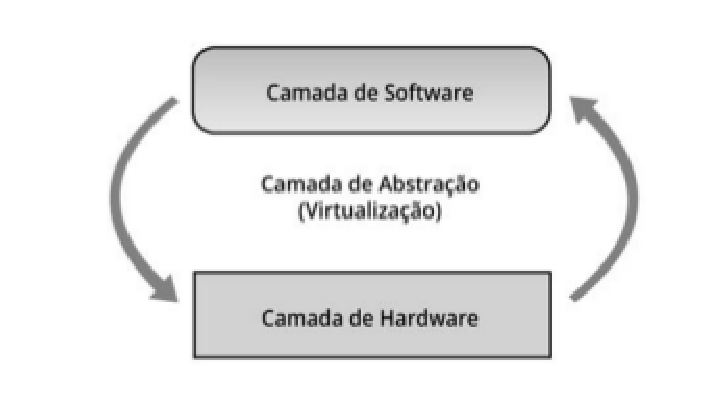
\includegraphics [keepaspectratio=true,scale=0.60]{figuras/virtualization_role.eps}
\caption{Responsabilidade da virtualização}
\cite{manoel}.
\label{virtualization_role}
\end{figure}

\subsection{Máquinas virtuais}
Uma máquina virtual é uma abstração em software de uma máquina física real. Destaca-se que é executada como uma aplicação padrão de usuário sobre um sistema operacional. A própria máquina virtual emula uma máquina física possuindo assim seus próprios discos e dispositivos \cite{}. Desse modo, umas das vantages de máquinas virtuais reside na independência de uso do seu sistmea operacional com relação ao sistema operacional da máquina física ao qual se encontra. Assim em uma máquina física pode-se executar várias máquinas virtuais cada uma delas com sistemas operacionais diversos. 
\subsection{Hipervisores}
O hipervisor (ou também conhecido como monitor de máquinas virtuais) é o software que possui mecanismos capazes de prover máquinas virtuais. Suas principais funções cosistem no esclanomaneto de tarefas, gerência da memória e manutenção do estado da máquina virtual \cite{manoel}. Desse modo, atributos como desempenho e escalabilidade são determinantes para definir a qualidade dos serviços fornecidos por um hipervisor. Algumas características são essenciais a um hipervisor: segurança sobre os recursos virtualizados e agilidade na reconfiguração de recursos computacionais, sem interromper as operações do servidor de máquinas virtuais \cite{manoel}. Os hipervisores são classificados em dois tipos:

\begin{itemize}
\item \textbf{Tipo I}(\textit{bare metal}, nativo ou supervisor):executa diretamente no hardware do sesrvidor. Controla o hardware e o acesso do sistema operacional convidado(\textit{guest OS}. O papel do hipervisor nativo é compartilhar os recursos de hardware entre as máquinas virtuais, de fomra que cada uma delas imagina ter recursos exclusivos \cite{manoel}.

\item \textbf{Tipo II}(hosted): aplicação que fornece um ambiente de execução para outras apicações. Executa sob um sistema operacional nativo como se fosse um processo deste. A camada de virtualização é composta por um sistema operacional hóspede e um hardware virtual, que são criados sobre os recursos de hardware oferecidos por meio do sistema operacional nativo \cite{manoel}.
\end{itemize}

\subsection{Tipos de virtualização}
A virtualização pode ser realizada de diferentes maneiras, cada uma com seus prós e contras. Na prática, em arquiteturas x86, as opções de virtualização alteram o nível de privilégios (\textit{rings}) padrões. As soluções baseads em hipervisores inclue a virtualização completa e a paravirtualização \cite{manoel}.

Na virtualização total, uma estrutura completa de hardware é virtualizada, portanto o sistema a ser virtualizado (sistema convidado) não precisa sofrer qualquer tipo de alteração. O principal benefícios da virtualização total é justamente o fato de que o sistema a ser virtualizado não sofre qualquer tipo de alteração \cite{marcos}. Entretanto, o sistema virtualizado eecuta de forma mais lenta e o monitor de máquinas virtuais precisa implementar alternativas para que as operações privilegidas possam ser executadas em procesadores que não suportem a virtualização nativamente \cite{marcos}.

\begin{figure}[!htb]
\centering
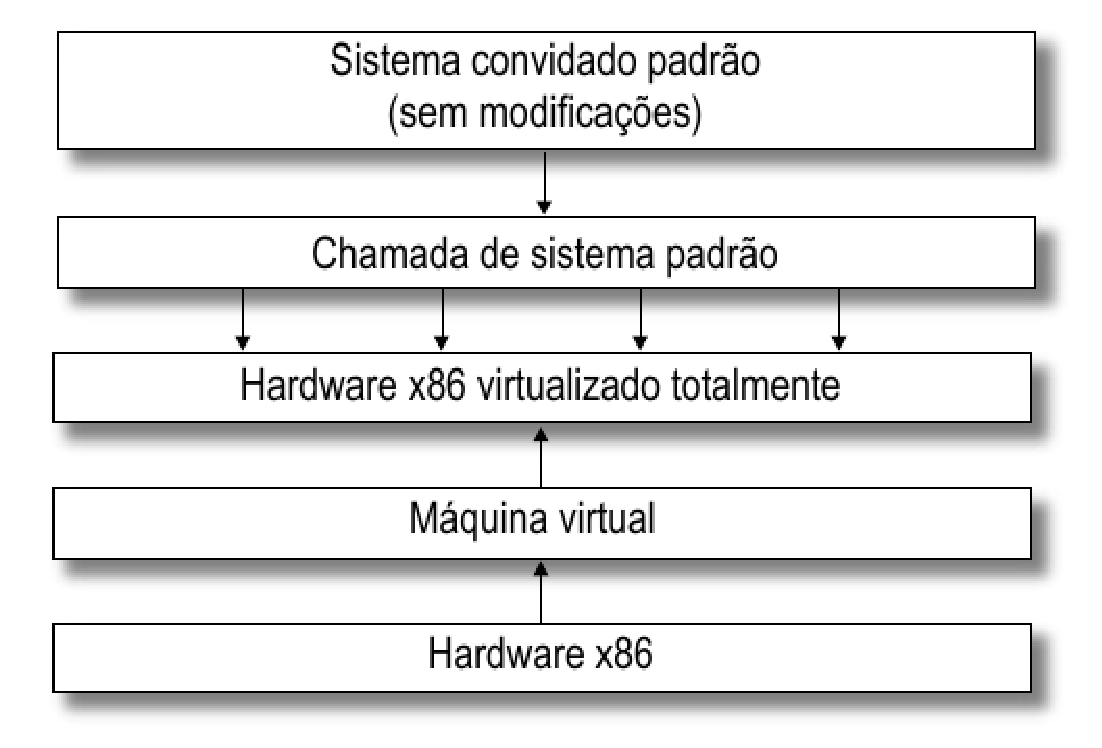
\includegraphics [keepaspectratio=true,scale=0.40]{figuras/full_virtualization.eps}
\caption{Representação da virtualização total}
\cite{marcos}.
\label{full_virtualization}
\end{figure}

Na paravirtualização, o sistema a ser virtualizado (sistema convidado) sofre modificações para que a interação com o monitor de máquinas virtuais seja mais eficiente. A paravirtualização permite que o sistema convidado consiga acesar recursos do hardware diretamente. O acesso é monitorado pelo monitor e máquinas virtuais, que ffornece ao sistema convidado todos os "limites" do sistema, tais como endereços de memória que podem ser utilizados e endereçamento em disco, por exemplo \cite{marcos}.

\begin{figure}[!htb]
\centering
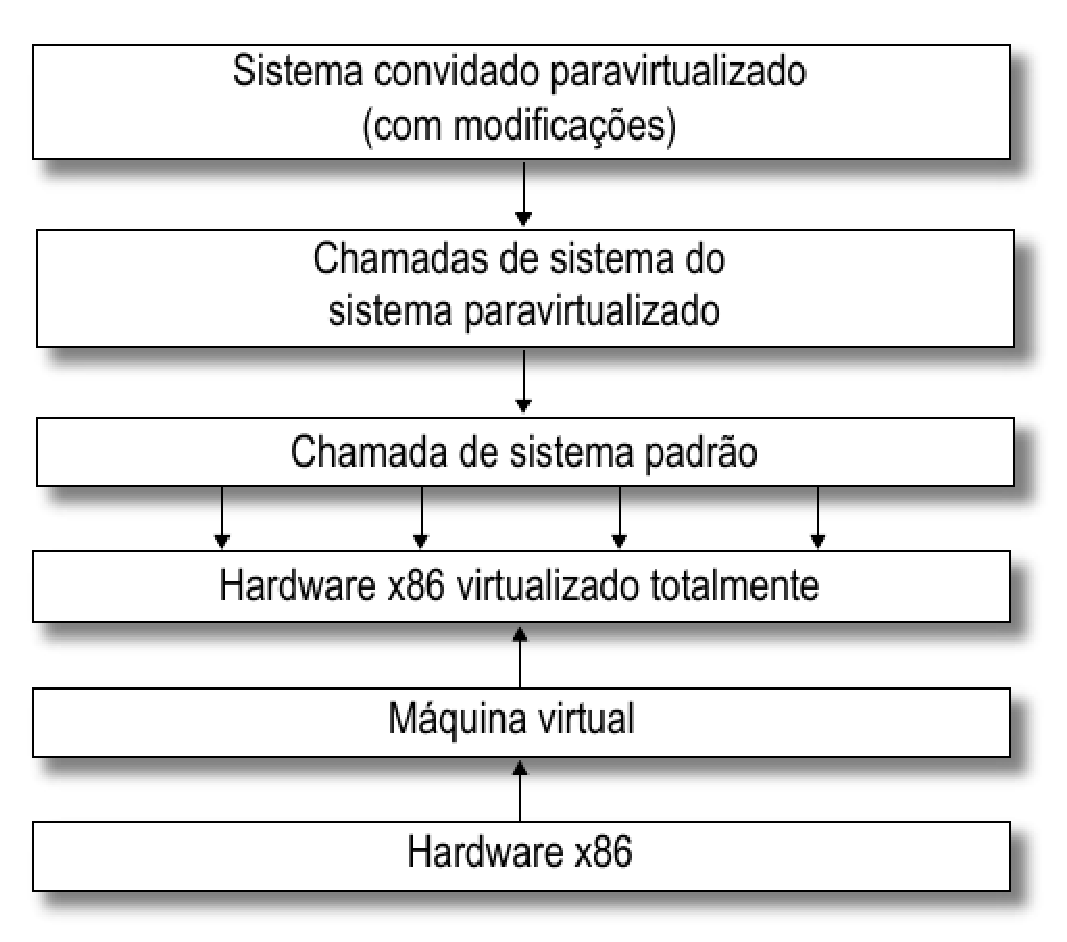
\includegraphics [keepaspectratio=true,scale=0.40]{figuras/paravirtualization.eps}
\caption{Representação da virtualização total}
\cite{marcos}.
\label{paravirtualization}
\end{figure}

\subsection{Ferramentas de Virtualização}
Nessa seção serão abordadas algumas das ferramentas principais utilizadas para provimento de ambientes virtualizados: \textit{Xen, KVM, VMMWare}
